\chapter{Introduction}
% \addcontentsline{toc}{chapter}{Introduction}



\section{JSON Schema}

Le JSON Schema \cite{JSON_Schema} est une norme permettant de décrire la structure et les contraintes des données au format JSON (JavaScript Object Notation). Il spécifie la manière dont les données JSON doivent être organisées, les types de données autorisés, les valeurs par défaut, etc.

\subsection{Utilité du JSON Schema}

\begin{enumerate}
    \item \textbf{Validation des données :} Il permet de valider si une instance JSON est conforme à un schéma prédéfini, assurant ainsi la qualité et la cohérence des données.
    
    \item \textbf{Documentation :} En décrivant la structure des données attendues, le JSON Schema sert également de documentation explicite pour les utilisateurs et les développeurs.
    
    \item \textbf{Communication :} En partageant un schéma, différentes parties prenantes peuvent avoir une compréhension commune de la structure des données, facilitant ainsi l'échange d'informations.
    
    \item \textbf{Génération de données de test :} Il peut être utilisé pour générer des jeux de données de test conformes au schéma, ce qui est utile lors de la phase de développement et de tests.
\end{enumerate}

\subsection{Intégration avec les Objectifs du Projet}

Dans le cadre du projet, les objectifs visent la génération et la correction d'instances JSON conformes à un schéma initial, tout en minimisant les modifications nécessaires. 

\begin{enumerate}
    \item \textbf{Validation initiale :} Les générateurs d'instances identifiés dans l'objectif 1 produisent des données JSON à partir des schémas. La première étape consiste à valider ces instances par rapport au JSON Schema, identifiant ainsi les non-conformités.
    
    \item \textbf{Réparation des instances :} L'objectif global du projet est de développer des approches de réparation permettant de minimiser les modifications nécessaires pour rendre une instance non conforme conforme au schéma initial.
    
    \item \textbf{Analyse des erreurs de validation :} L'objectif 4 consiste à étudier le lien entre les erreurs de validation, détectées à l'étape 1, et la distance d'édition entre les instances non conformes et l'instance valide. Cette analyse contribue à une compréhension approfondie des types d'erreurs et guide le processus de réparation.
\end{enumerate}
\section{La similarité des documents JSON}
La similarité des documents JSON est une mesure de la similarité entre deux documents JSON. Elle est généralement utilisée pour comparer des documents JSON qui représentent des objets ou des données similaires.
\subsection{Approches existantes}
Une des approches existantes pour calculer la similarité des documents JSON est :
\begin{itemize}
    \item [\textbullet] \textbf{Approche top-down \cite{JSON_Similarity}:} 
Cet approche top-down pour un comparateur de similarité dans le contexte JSON consiste à examiner la similarité entre deux structures JSON en commençant par les éléments les plus généraux et en descendant progressivement vers les détails spécifiques. Cela implique une comparaison basée sur la hiérarchie des éléments plutôt que sur les valeurs individuelles. ensuite les valeurs des propriétés et des éléments des deux documents.
\end{itemize}
\subsection{Limitations :}
\begin{enumerate}
    \item \textbf{La structure du document est ignorée :} les approches top-down ignorent la structure du document, ce qui peut conduire à des résultats inexacts.
    \item \textbf{Aucune garantie de qualité n'est donnée :} les approches existantes ne fournissent généralement aucune garantie de qualité pour leurs résultats.
\end{enumerate}
\section{JEDI}
JEDI \cite{JEDI} est un algorithme de calcul de la similarité entre deux documents JSON. Il fonctionne en comparant les deux documents en tant qu'arbres. La similarité entre les deux documents est définie comme le nombre minimum d'opérations d'édition (Ajout, Suppression, Modification) nécessaires pour transformer un arbre en l'autre. 
\begin{figure}[H]
    \centering
    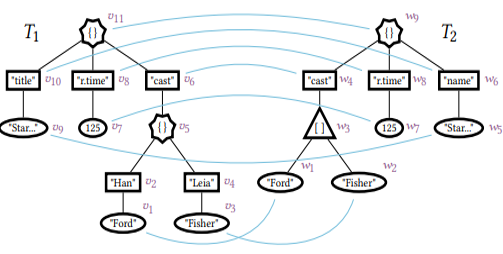
\includegraphics{Photos/Tree.png}
    \caption{\cite{JEDI}}

\end{figure}
\subsection{Principe de calcul de similarités de JEDI}
A partir d'un \textbf{Treshold} \textbf{T} et des documents \textbf{$d_{q}$}, on veut extraire à partir d’une base de données \textbf{D} les documents \textbf{$d_{i}$} qui sont similaires ( \textbf{JEDI} (\textbf{$d_{q}$} ,\textbf{$d_{i}$}) < \textbf{T} ). La solution proposée est donc de complexité \textbf{O($n^{2}\times d \times \log(d)$)} avec \textbf{n} étant la taille de l'arbre et \textbf{d} le degré maximum de l'arbre. 
\subsubsection{QuickJedi}
L'algorithme JEDI est complexe et peut être lent pour traiter de grandes quantités de données. Pour réduire le temps de calcul, il est donc indisponsable de filtrer les documents avant de les comparer à l'aide de JEDI. Le filtrage consiste à sélectionner les documents les plus susceptibles d'être similaires à la requête. Une fois les documents filtrés, l'algorithme JEDI peut être utilisé pour calculer la similarité entre les documents candidats.

\begin{figure}[H]
    \centering
    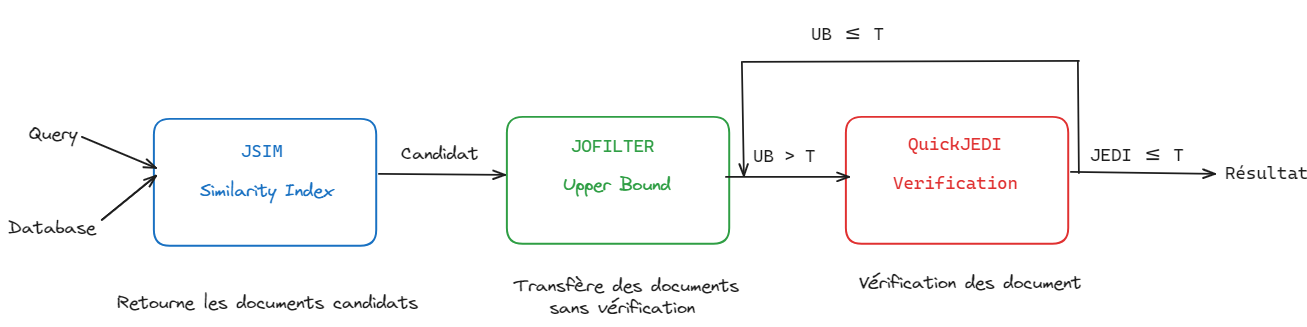
\includegraphics[width=\linewidth]{Photos/QuickJedi.PNG}
    \caption{\cite{JEDI}}

\end{figure}